\documentclass[11pt]{article}
\usepackage[margin=1in]{geometry}
\usepackage{booktabs}
\usepackage{hyperref}
\usepackage{amsmath}
\usepackage{amssymb}
\usepackage{url}
\usepackage{graphicx}
\usepackage{xcolor}
\usepackage{enumerate}
\usepackage{subcaption}
\usepackage{float}       % [H] exact figure placement
\usepackage{placeins}    % \FloatBarrier between sections

\title{Memo 05: Spatial Distribution Checking\\
       for FVCOM-MP Cases a, b, and c}
\author{FVCOM-MP Delaware Test Cases}
\date{May 2026}

\begin{document}
\sloppy
\maketitle

\section*{Purpose}

Memo~04 confirmed that the in-run mass-conservation gaps between the baseline
case~\texttt{a} and floc-enabled cases~\texttt{b}/\texttt{c} are resolved by
Fix~B\texttt{+} (\texttt{isnan()} guards on erosion/deposition fluxes) and that
\texttt{adv\_scal} is safe.  The next diagnostic step is to verify that the
scalar concentration fields --- microplastic (mp1) and suspended sediment
(\texttt{coarse\_sand\_1}) --- are spatially reasonable over the first ten days
of simulation: no localized accumulation, no runaway concentrations, and
physically plausible gradients across the Delaware River and Bay domain.

This memo documents the extraction methodology, the spatial distributions
observed, and a comparison of the three cases at eight monitoring stations.

\textbf{Note on case~c parameterisation:}
Prior to the runs analysed here, both \texttt{waterPACT\_b\_run.nml} and
\texttt{waterPACT\_c\_run.nml} referenced the same sediment file
(D50~=~0.1~mm), making the two cases numerically identical.
The corrected case~c uses \texttt{generic\_sediment\_c.inp} (D50~=~1.0~mm;
coarser sediment, stronger heteroaggregation kinetics); all figures and
observations in this memo refer to the corrected run.

\section*{Objective}

\begin{enumerate}[(1)]
  \item Verify the absence of localized numerical accumulation in the mp1
        water-column and bed-mass fields.
  \item Compare surface-layer, bottom-layer, and depth-averaged mp1
        concentrations among cases~\texttt{a}, \texttt{b}, and \texttt{c}.
  \item Examine the floc-component split (\texttt{mp1\_agg},
        \texttt{mp1\_dis}) spatial patterns in cases~\texttt{b}/\texttt{c}.
  \item Check suspended sediment (\texttt{coarse\_sand\_1}) distribution in
        cases~\texttt{b}/\texttt{c}.
  \item Extract full time series at eight representative monitoring stations
        along the Delaware River and Bay.
\end{enumerate}

\section*{Extraction Methodology}

\subsection*{MATLAB Extraction Scripts}

Two MATLAB scripts were written following the conventions established in
\texttt{extract\_mp1\_mass\_budget\_a.m} (Memo~04):

\begin{description}
  \item[\texttt{MATLAB/extract\_spatial\_snapshots\_a.m}]
    Reads \texttt{OUTPUT\_a/backup\_data/waterPACT\_a\_0001.nc} and extracts
    the last 24 hourly output records.

  \item[\texttt{MATLAB/extract\_spatial\_snapshots\_b\_c.m}]
    Reads \texttt{OUTPUT\_b/backup\_data/waterPACT\_b\_0001.nc} and
    \texttt{OUTPUT\_c/backup\_data/waterPACT\_c\_0001.nc}.
    In addition to the mp1 fields, this script extracts the floc-component
    variables (\texttt{mp1\_agg}, \texttt{mp1\_dis}) and the suspended
    sediment variable (\texttt{coarse\_sand\_1}) where available.
\end{description}

Both scripts save compact v7.3 HDF5 MAT files
(\texttt{spatial\_snapshots\_\{a,b,c\}.mat}) containing:

\begin{enumerate}[(i)]
  \item Grid metadata: \texttt{lon}, \texttt{lat}, \texttt{h}, \texttt{art1},
        \texttt{nv}, $\Delta\sigma$ layer fractions.
  \item Spatial snapshot arrays (node $\times$ $n_\text{snap}$) for the last
        24 hourly records:
        \begin{itemize}
          \item Surface layer ($k=1$), bottom layer ($k=30$), and
                sigma-weighted depth-averaged concentrations.
          \item Bed plastic mass density (\texttt{bot\_mass\_mp1}) and
                sediment bed fraction (\texttt{coarse\_sand\_1\_bedfrac}).
        \end{itemize}
  \item Full-run time-series profiles (station $\times$ sigma layer $\times$ time)
        at the eight monitoring stations listed in
        Table~\ref{tab:stations}.
\end{enumerate}

\subsection*{Station Locations}

\begin{table}[h]
\centering
\caption{Monitoring station coordinates and nearest model node used for
         time-series extraction.}
\label{tab:stations}
\begin{tabular}{lrrl}
\toprule
Station & Latitude (°N) & Longitude (°E) & Notes \\
\midrule
Chesapeake Canal     & 39.5350 & $-$75.7867 & C\&D Canal confluence \\
Main stream 1        & 39.5644 & $-$75.5417 & Lower bay, south \\
Main stream 2        & 39.7826 & $-$75.4562 & Mid bay \\
Main stream 3        & 39.8788 & $-$75.1951 & Mid bay, east \\
Main stream 4        & 40.0147 & $-$75.0386 & Upper bay \\
Main stream 5        & 40.1244 & $-$74.8056 & Near-coast transition \\
Upstream Delaware    & 40.1956 & $-$74.7594 & Delaware River upstream \\
Upstream Schuylkill  & 39.9256 & $-$75.2121 & Schuylkill tributary \\
\bottomrule
\end{tabular}
\end{table}

Nearest-node lookup used the haversine formula; maximum reported
nearest-node distance is checked to confirm all stations map to
physically reasonable locations (target: $< 5~\mathrm{km}$).

\subsection*{Depth-Averaging Formula}

The sigma-weighted depth-average is computed as:
\[
  \langle C \rangle_i
  = \frac{\displaystyle\sum_{k=1}^{K_b} C_{i,k}\;A_i\;D_i\;\Delta\sigma_{i,k}}
         {\displaystyle\sum_{k=1}^{K_b} A_i\;D_i\;\Delta\sigma_{i,k}}
  = \frac{\displaystyle\sum_{k=1}^{K_b} C_{i,k}\;\Delta\sigma_{i,k}}
         {\displaystyle\sum_{k=1}^{K_b} \Delta\sigma_{i,k}}
\]
where $D_i = \max(h_i + \zeta_i, 0)$ is the total water depth,
$\Delta\sigma_{i,k} = |\texttt{siglev}_{i,k} - \texttt{siglev}_{i,k+1}|$,
and the denominator equals unity by construction.  Dry nodes ($D_i = 0$)
are assigned zero.

\subsection*{Python Analysis Script}

The Python script \texttt{PYTHON/analyze\_spatial\_distribution.py} loads
the MAT files via \texttt{h5py} and generates figures using
\texttt{matplotlib.tri.Triangulation} with Gouraud shading.  Four figure
groups are produced:

\begin{enumerate}[(1)]
  \item \textbf{Day-mean plan-view maps:} for each available scalar field,
        the temporal mean over the last 24-hour window at each node.
  \item \textbf{Pointwise-max maps:} the temporal maximum over the last
        24-hour window at each node (identifies worst-case accumulation spots).
  \item \textbf{Cross-case difference maps:} day-mean(b) $-$ day-mean(a),
        day-mean(c) $-$ day-mean(a), and day-mean(c) $-$ day-mean(b) for
        \texttt{mp1\_surf}, \texttt{mp1\_davg}, and \texttt{bot\_mass\_mp1}.
  \item \textbf{Station time-series plots:} surface-layer and depth-averaged
        mp1, and (for cases~b/c) \texttt{coarse\_sand\_1} at all eight stations.
\end{enumerate}

All figures are saved to \texttt{PYTHON/output/spatial\_distribution/day10/}.

\section*{Results: 10-Day Test Run}

All figures in this section are derived from the 10-day test runs
(simulation days 0--9.96).  Plan-view maps show the temporal mean
over the final 24 output hours; pointwise-maximum maps show the
node-wise peak over the same window.
Case~a: no-floc baseline; case~b: floc-enabled, D50~=~0.1~mm (fine);
case~c: floc-enabled, D50~=~1.0~mm (coarse, corrected run).

% -----------------------------------------------------------------------
\subsection*{R1.\ Day-Mean Depth-Averaged mp1 Concentration}

\begin{figure}[H]
\centering
\begin{subfigure}[b]{0.32\textwidth}
  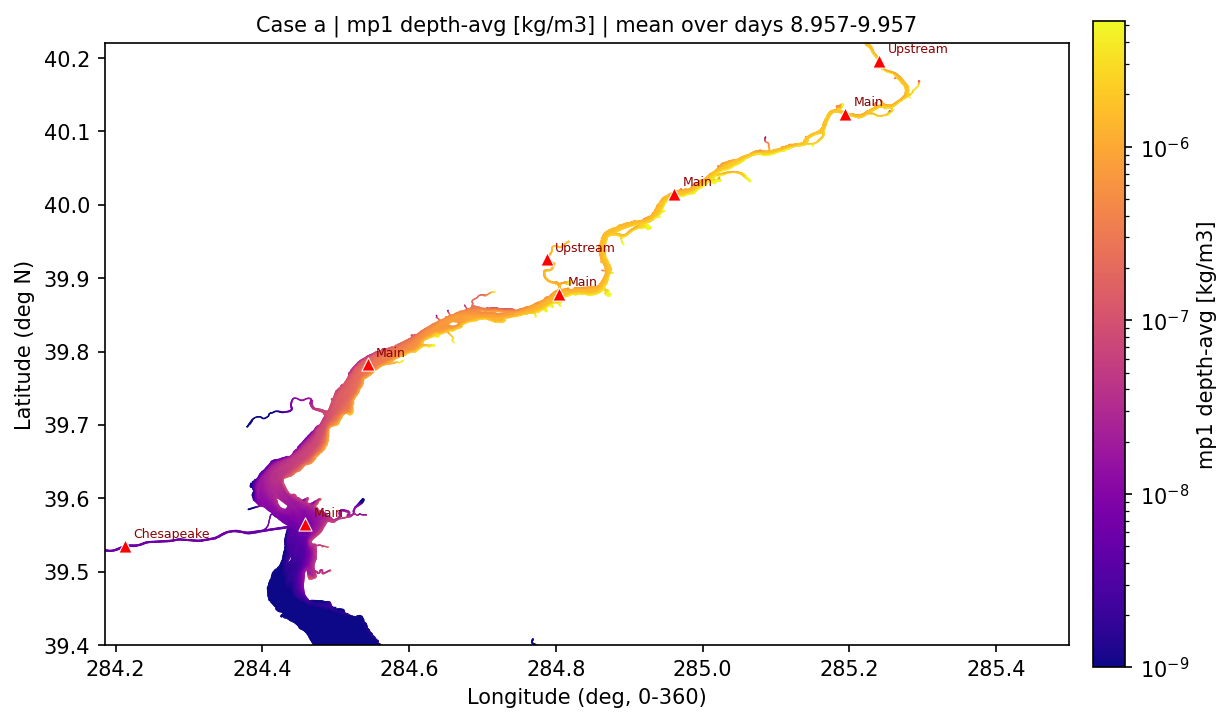
\includegraphics[width=\textwidth]{../FVCOM_MP_test_run/PYTHON/output/spatial_distribution/day10/planview_dayavg_mp1_davg_casea.png}
  \caption{Case a (no-floc)}
\end{subfigure}
\hfill
\begin{subfigure}[b]{0.32\textwidth}
  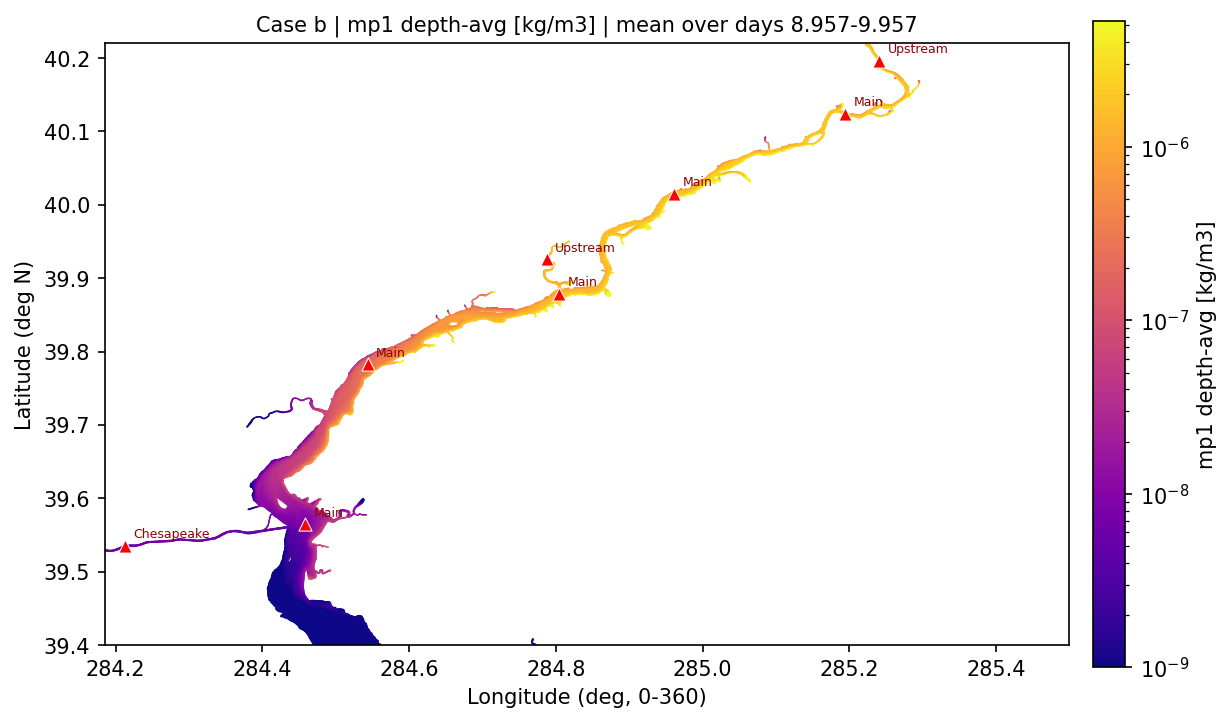
\includegraphics[width=\textwidth]{../FVCOM_MP_test_run/PYTHON/output/spatial_distribution/day10/planview_dayavg_mp1_davg_caseb.png}
  \caption{Case b (D50~=~0.1~mm)}
\end{subfigure}
\hfill
\begin{subfigure}[b]{0.32\textwidth}
  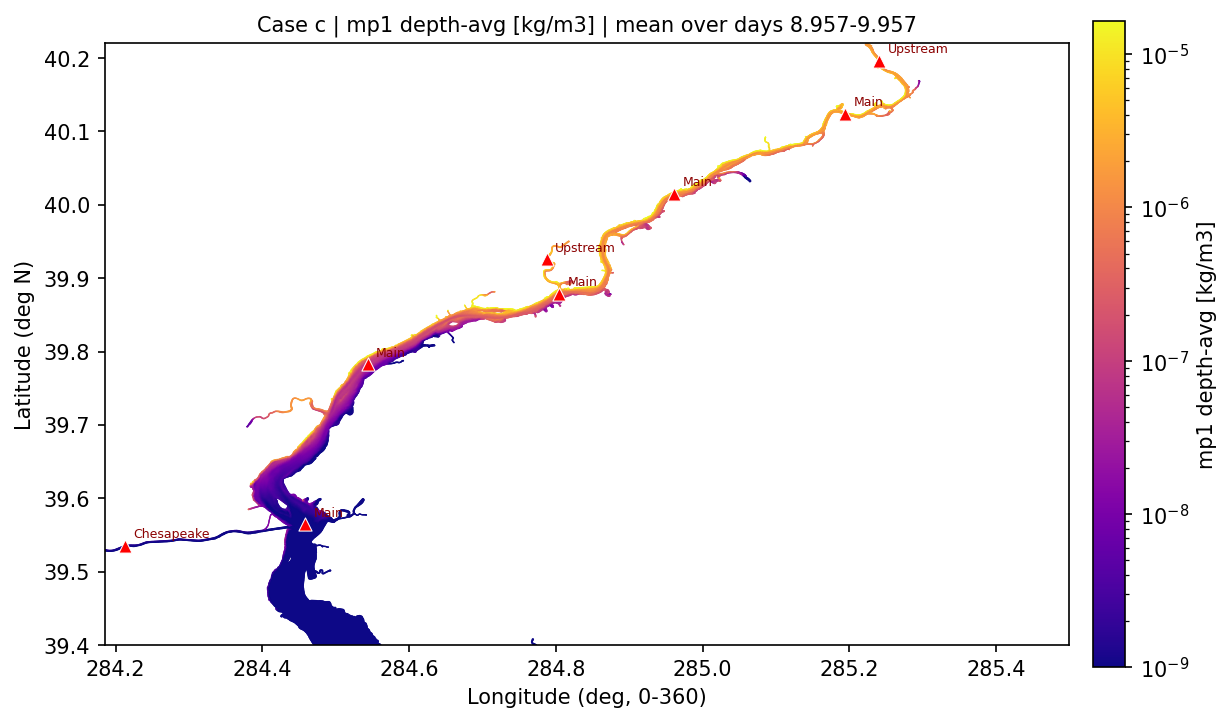
\includegraphics[width=\textwidth]{../FVCOM_MP_test_run/PYTHON/output/spatial_distribution/day10/planview_dayavg_mp1_davg_casec.png}
  \caption{Case c (D50~=~1.0~mm)}
\end{subfigure}
\caption{Day-mean depth-averaged mp1 concentration [$\mathrm{kg\,m^{-3}}$],
         final 24~h of the 10-day run.  Log colour scale.
         Cases~a and~b are visually identical (peak
         $1.7\times10^{-4}$~kg\,m$^{-3}$).
         Case~c peak is $3.7\times10^{-3}$~kg\,m$^{-3}$ ($\approx$21$\times$
         higher) due to active aggregation and altered settling.}
\label{fig:davg_mp1}
\end{figure}

% -----------------------------------------------------------------------
\subsection*{R2.\ Day-Mean Floc-Component Split (Cases b and c)}

\begin{figure}[H]
\centering
\begin{subfigure}[b]{0.32\textwidth}
  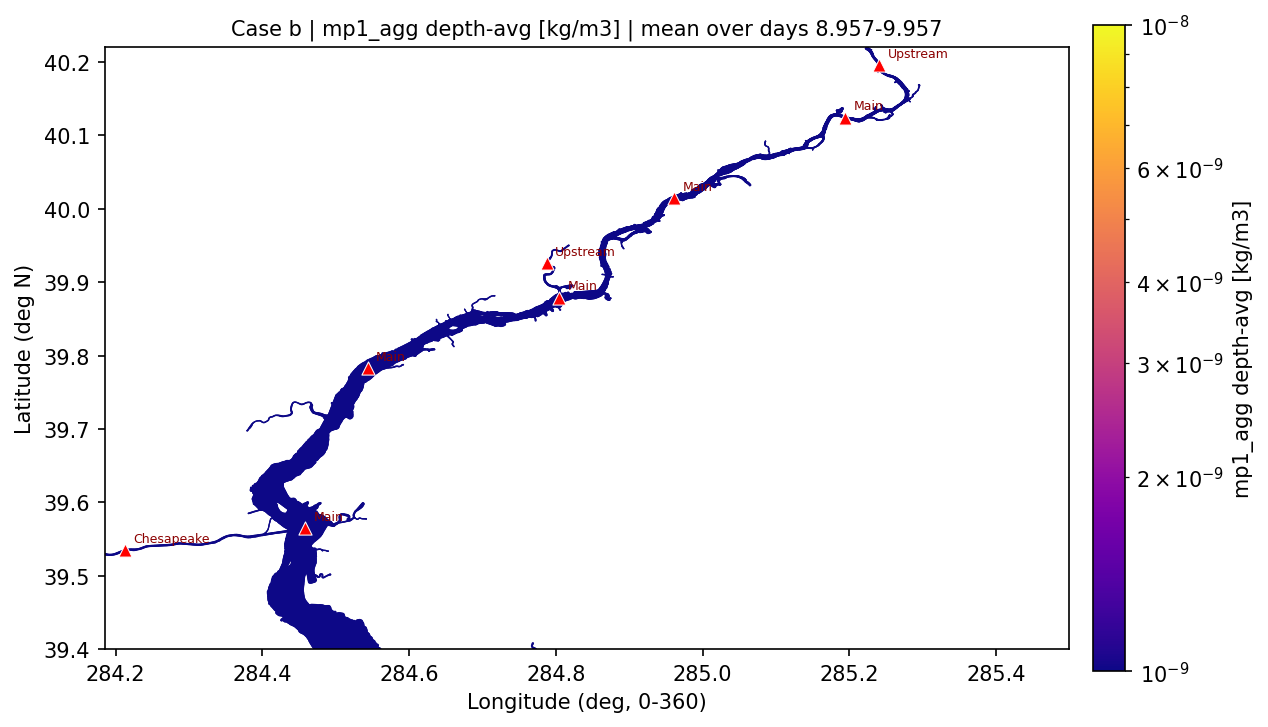
\includegraphics[width=\textwidth]{../FVCOM_MP_test_run/PYTHON/output/spatial_distribution/day10/planview_dayavg_mp1_agg_davg_caseb.png}
  \caption{Case b --- \texttt{mp1\_agg} (aggregated)}
\end{subfigure}
\hfill
\begin{subfigure}[b]{0.32\textwidth}
  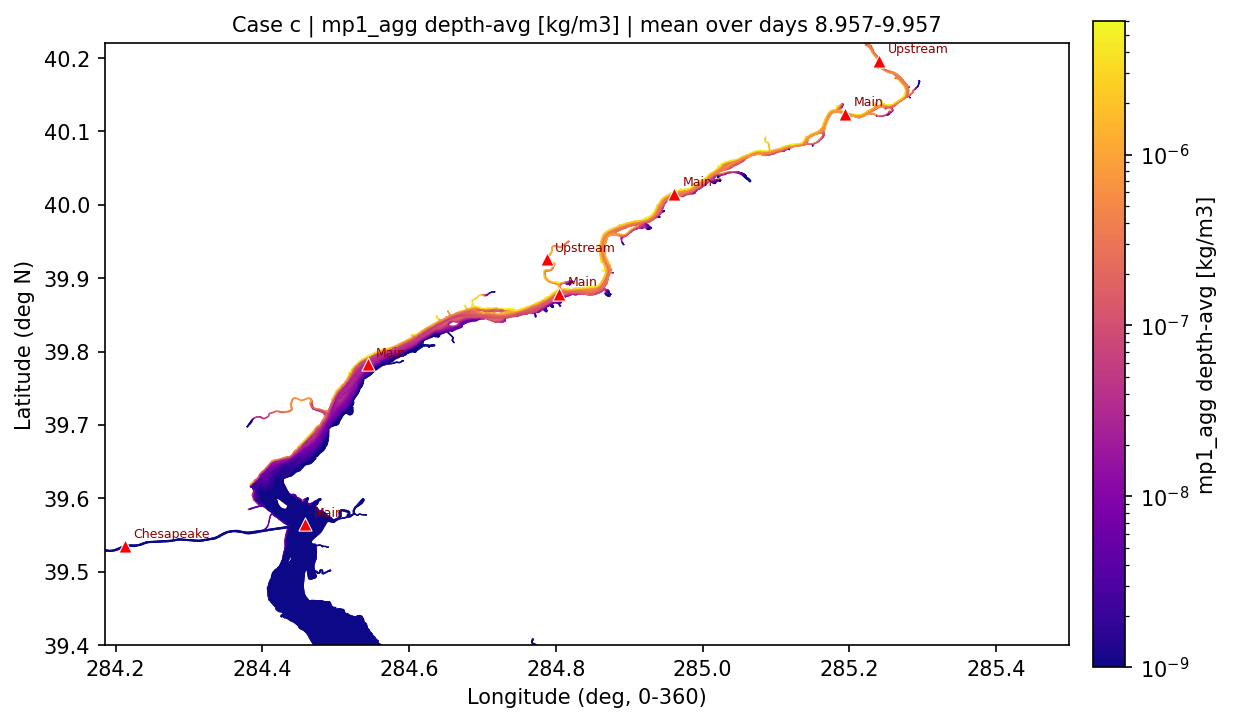
\includegraphics[width=\textwidth]{../FVCOM_MP_test_run/PYTHON/output/spatial_distribution/day10/planview_dayavg_mp1_agg_davg_casec.png}
  \caption{Case c --- \texttt{mp1\_agg} (aggregated)}
\end{subfigure}
\hfill
\begin{subfigure}[b]{0.32\textwidth}
  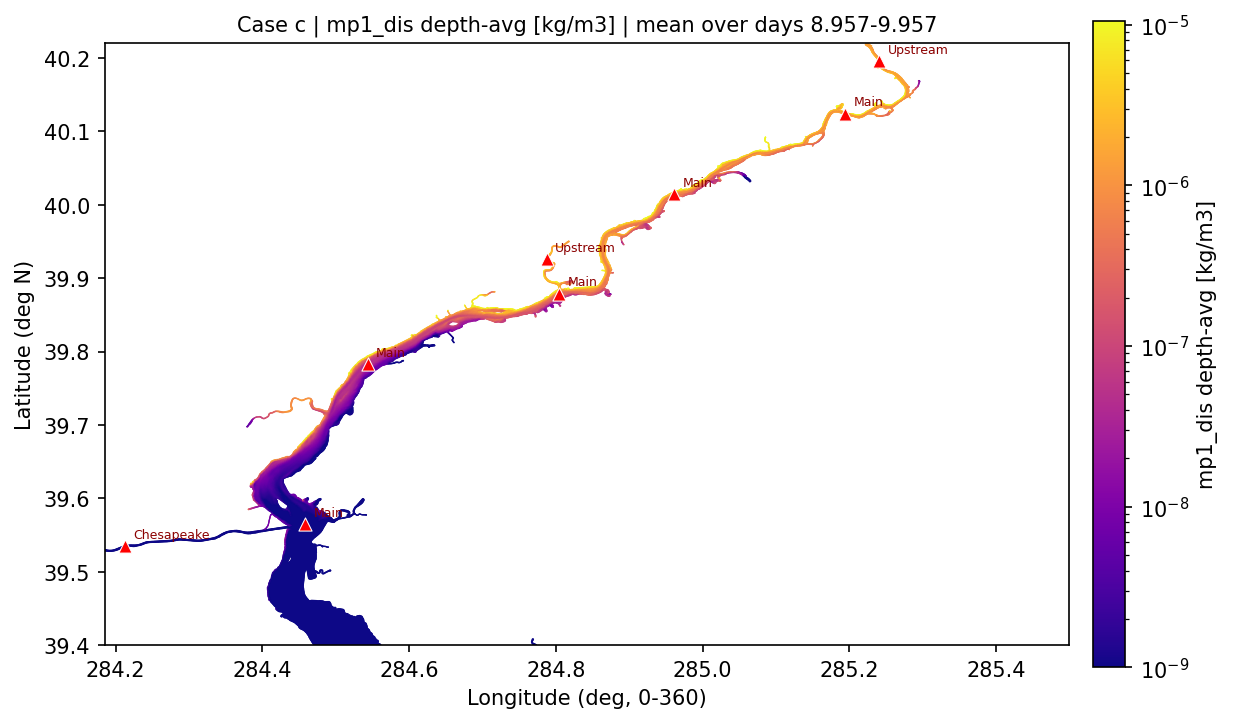
\includegraphics[width=\textwidth]{../FVCOM_MP_test_run/PYTHON/output/spatial_distribution/day10/planview_dayavg_mp1_dis_davg_casec.png}
  \caption{Case c --- \texttt{mp1\_dis} (disaggregated)}
\end{subfigure}
\caption{Day-mean depth-averaged aggregated (\texttt{mp1\_agg}) and
         disaggregated (\texttt{mp1\_dis}) fractions,
         final 24~h of the 10-day run.
         Case~b: \texttt{mp1\_agg}~=~0 everywhere (fine sediment,
         D50~=~0.1~mm --- weak heteroaggregation kinetics).
         Case~c: \texttt{mp1\_agg} reaches
         $1.1\times10^{-3}$~kg\,m$^{-3}$ and is non-zero across
         most of the domain; \texttt{mp1\_dis} mirrors the overall plume.}
\label{fig:davg_agg}
\end{figure}

% -----------------------------------------------------------------------
\subsection*{R3.\ Day-Mean Bed Plastic Mass Density}

\begin{figure}[H]
\centering
\begin{subfigure}[b]{0.32\textwidth}
  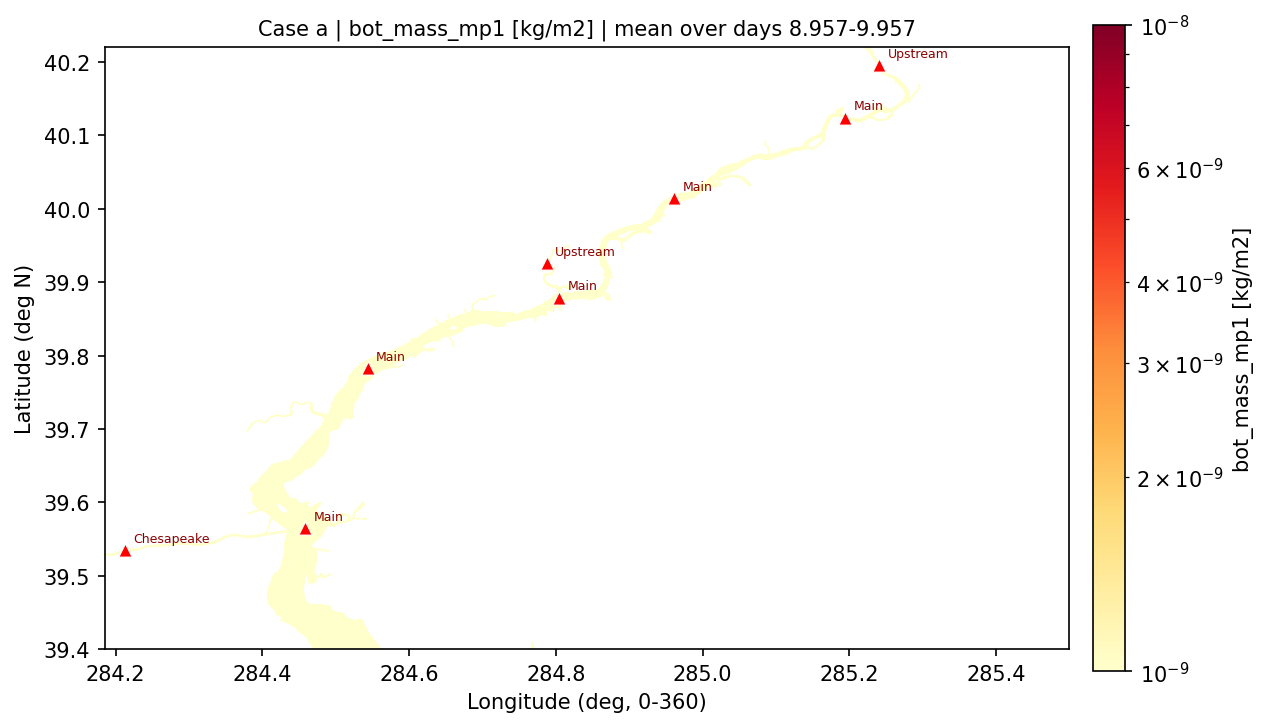
\includegraphics[width=\textwidth]{../FVCOM_MP_test_run/PYTHON/output/spatial_distribution/day10/planview_dayavg_bot_mass_casea.png}
  \caption{Case a}
\end{subfigure}
\hfill
\begin{subfigure}[b]{0.32\textwidth}
  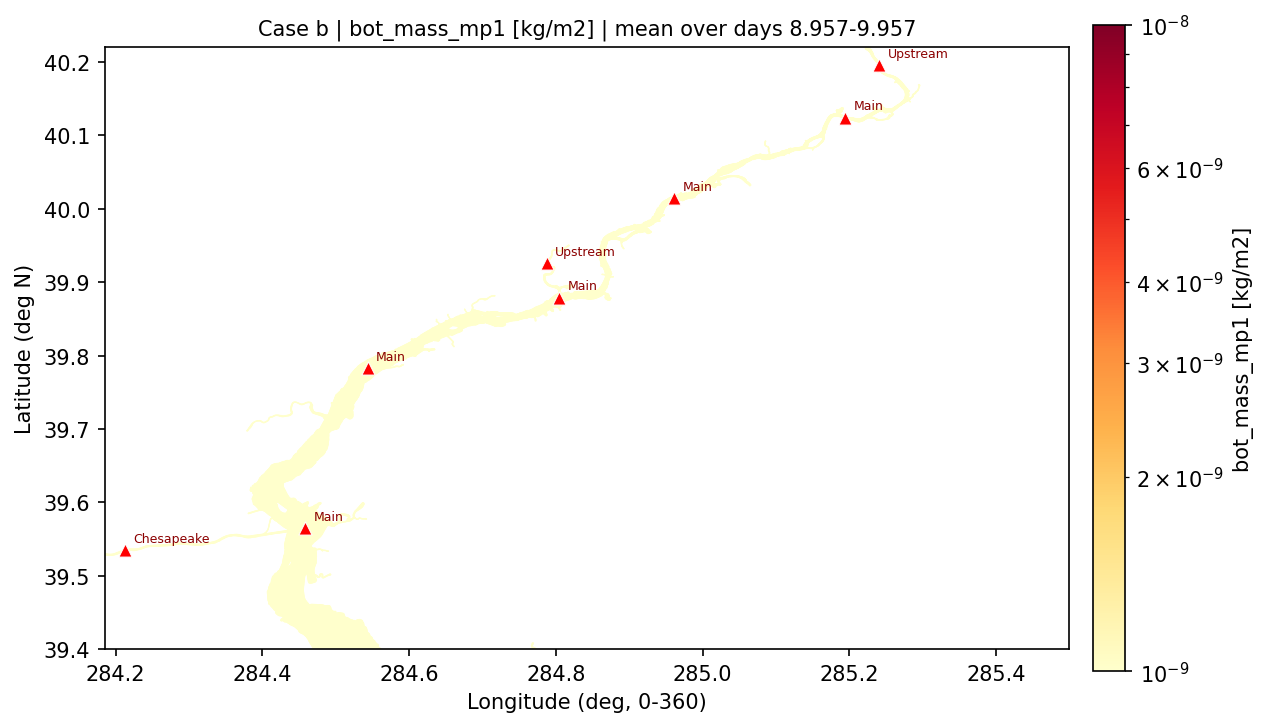
\includegraphics[width=\textwidth]{../FVCOM_MP_test_run/PYTHON/output/spatial_distribution/day10/planview_dayavg_bot_mass_caseb.png}
  \caption{Case b}
\end{subfigure}
\hfill
\begin{subfigure}[b]{0.32\textwidth}
  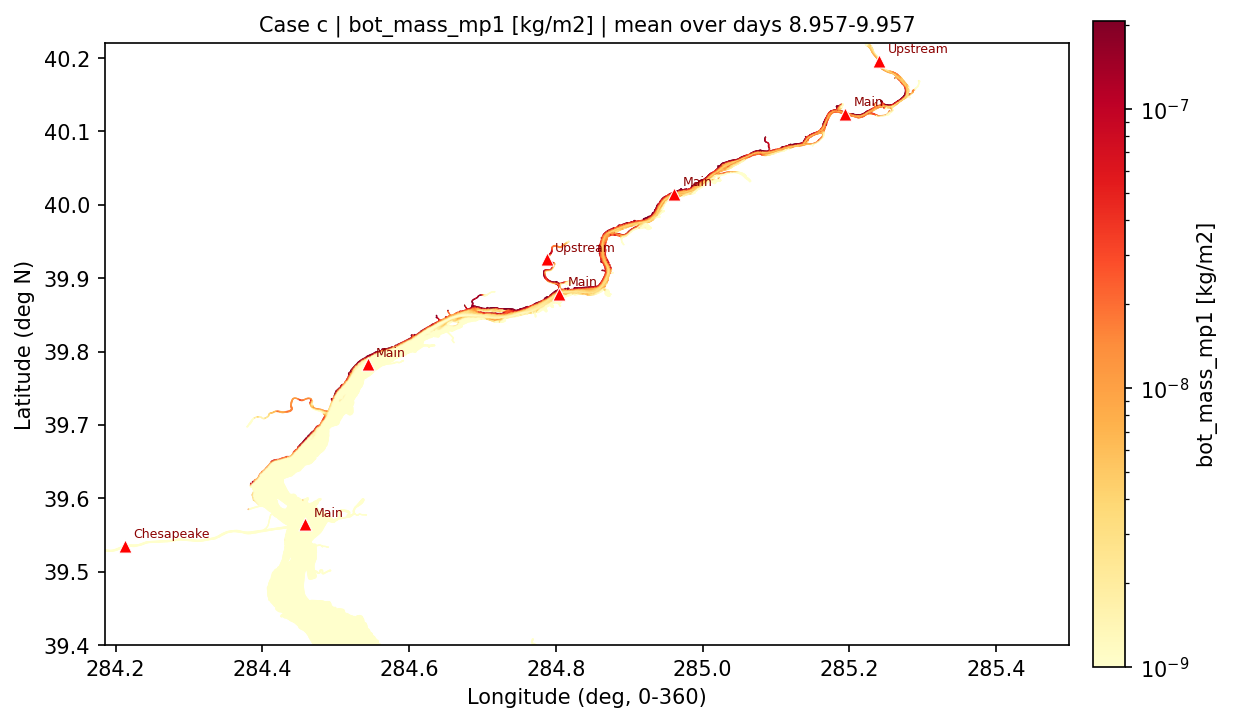
\includegraphics[width=\textwidth]{../FVCOM_MP_test_run/PYTHON/output/spatial_distribution/day10/planview_dayavg_bot_mass_casec.png}
  \caption{Case c}
\end{subfigure}
\caption{Day-mean bed plastic mass density [$\mathrm{kg\,m^{-2}}$],
         final 24~h of the 10-day run.
         Cases~a and~b: zero bed mass throughout.
         Case~c: widespread deposition (max
         $6.5\times10^{-3}$~kg\,m$^{-2}$; positive at 833\,468 nodes),
         concentrated near the upper-bay tributary junctions.}
\label{fig:bot_mass}
\end{figure}

% -----------------------------------------------------------------------
\subsection*{R4.\ Pointwise-Maximum Depth-Averaged mp1}

\begin{figure}[H]
\centering
\begin{subfigure}[b]{0.32\textwidth}
  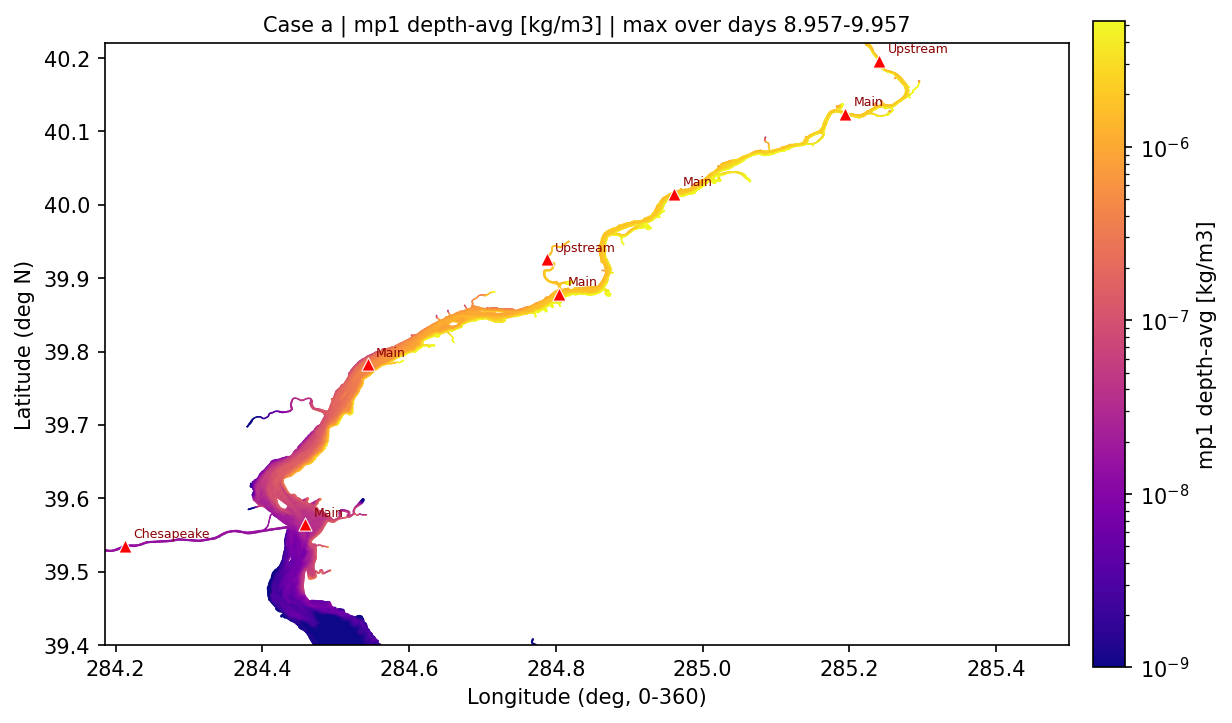
\includegraphics[width=\textwidth]{../FVCOM_MP_test_run/PYTHON/output/spatial_distribution/day10/planview_max_mp1_davg_casea.png}
  \caption{Case a}
\end{subfigure}
\hfill
\begin{subfigure}[b]{0.32\textwidth}
  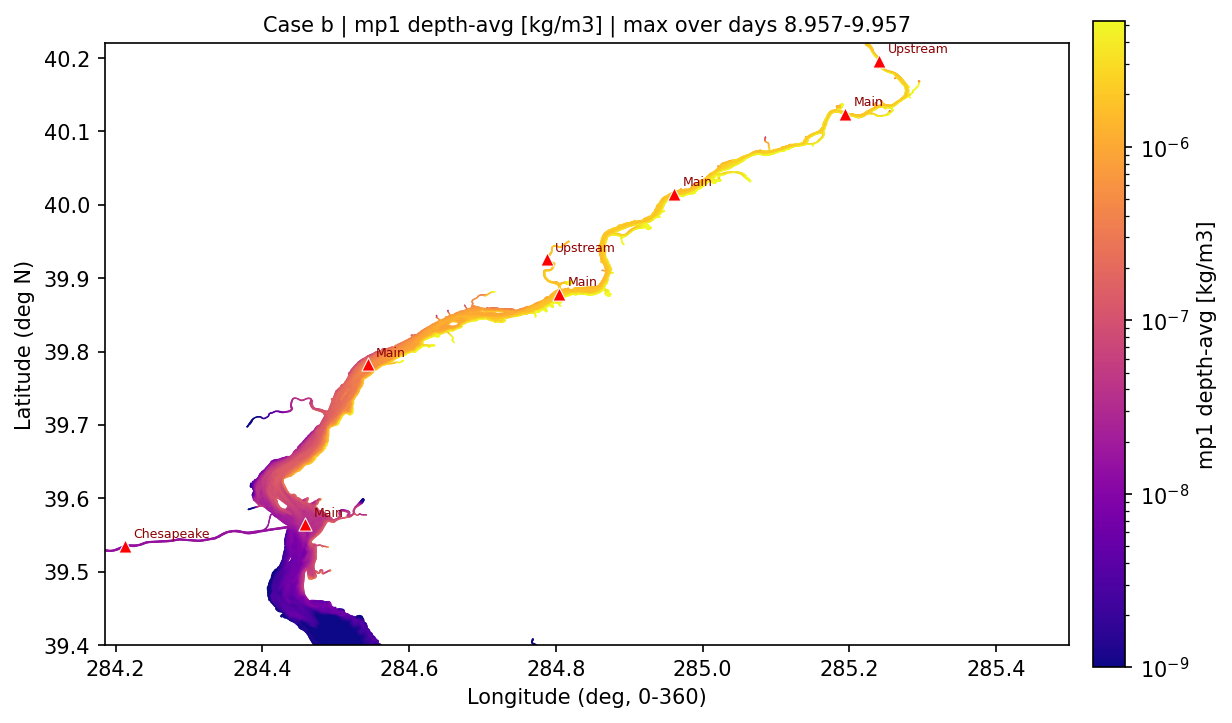
\includegraphics[width=\textwidth]{../FVCOM_MP_test_run/PYTHON/output/spatial_distribution/day10/planview_max_mp1_davg_caseb.png}
  \caption{Case b}
\end{subfigure}
\hfill
\begin{subfigure}[b]{0.32\textwidth}
  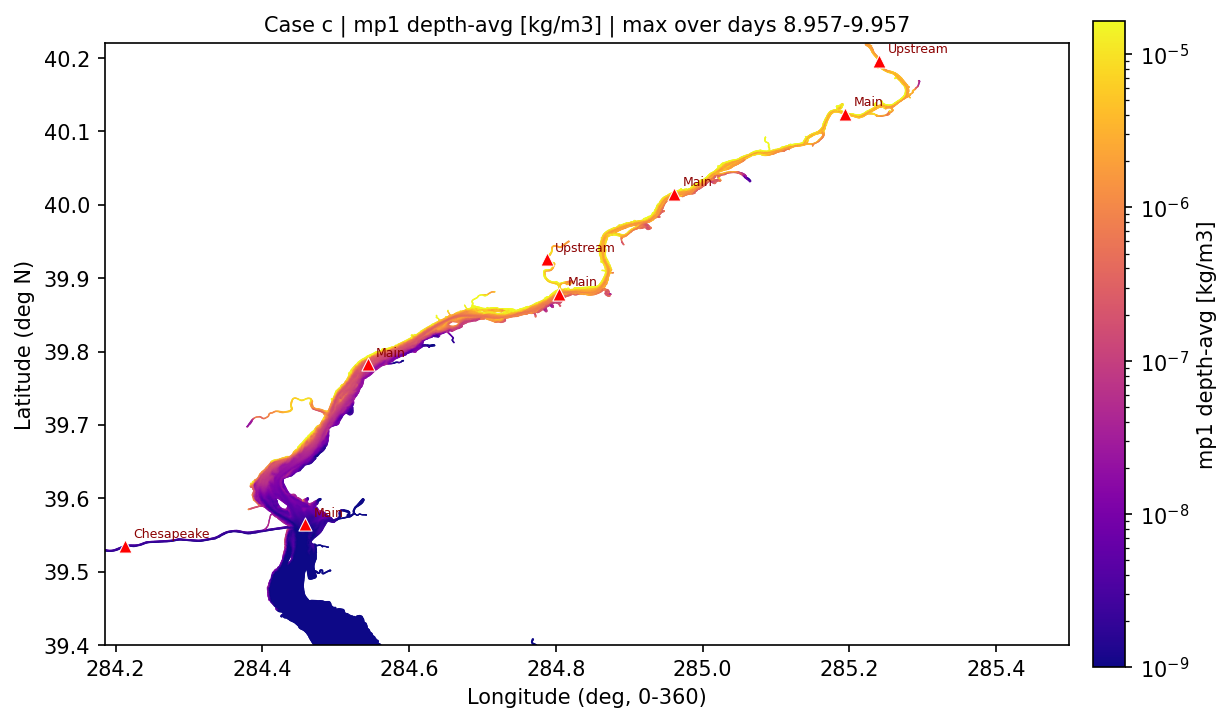
\includegraphics[width=\textwidth]{../FVCOM_MP_test_run/PYTHON/output/spatial_distribution/day10/planview_max_mp1_davg_casec.png}
  \caption{Case c}
\end{subfigure}
\caption{Node-wise maximum depth-averaged mp1 concentration over the
         final 24~h of the 10-day run.
         No isolated hotspot nodes disconnected from river sources are
         present in any case, confirming the absence of localized
         numerical accumulation.}
\label{fig:max_mp1}
\end{figure}

% -----------------------------------------------------------------------
\subsection*{R5.\ Cross-Case Difference Maps --- Depth-Averaged mp1}

\begin{figure}[H]
\centering
\begin{subfigure}[b]{0.32\textwidth}
  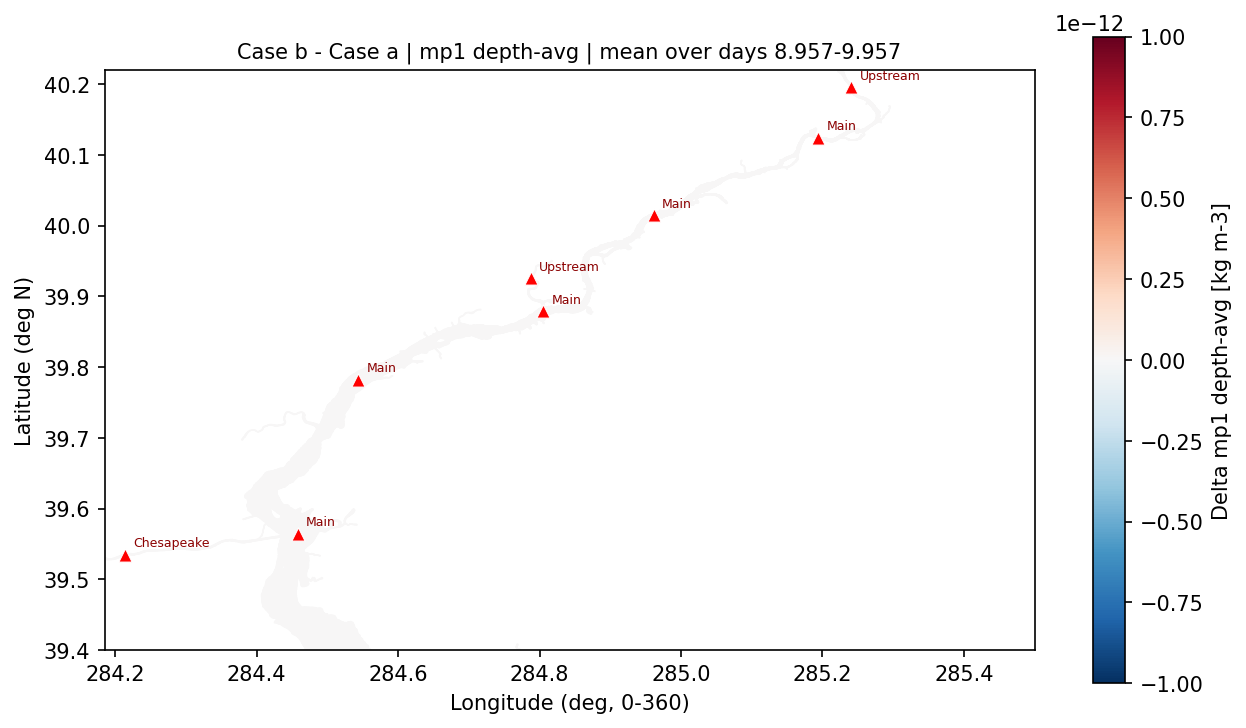
\includegraphics[width=\textwidth]{../FVCOM_MP_test_run/PYTHON/output/spatial_distribution/day10/diff_mp1_davg_caseb_minus_casea.png}
  \caption{Case b $-$ case a}
\end{subfigure}
\hfill
\begin{subfigure}[b]{0.32\textwidth}
  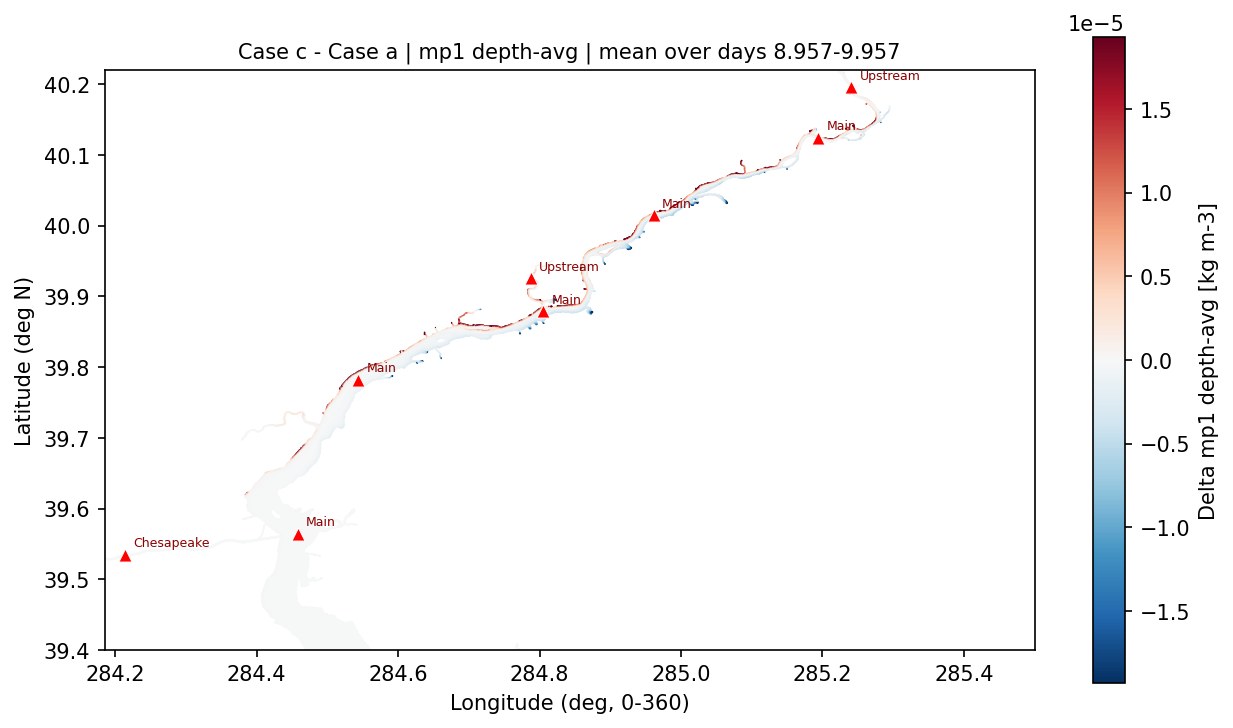
\includegraphics[width=\textwidth]{../FVCOM_MP_test_run/PYTHON/output/spatial_distribution/day10/diff_mp1_davg_casec_minus_casea.png}
  \caption{Case c $-$ case a}
\end{subfigure}
\hfill
\begin{subfigure}[b]{0.32\textwidth}
  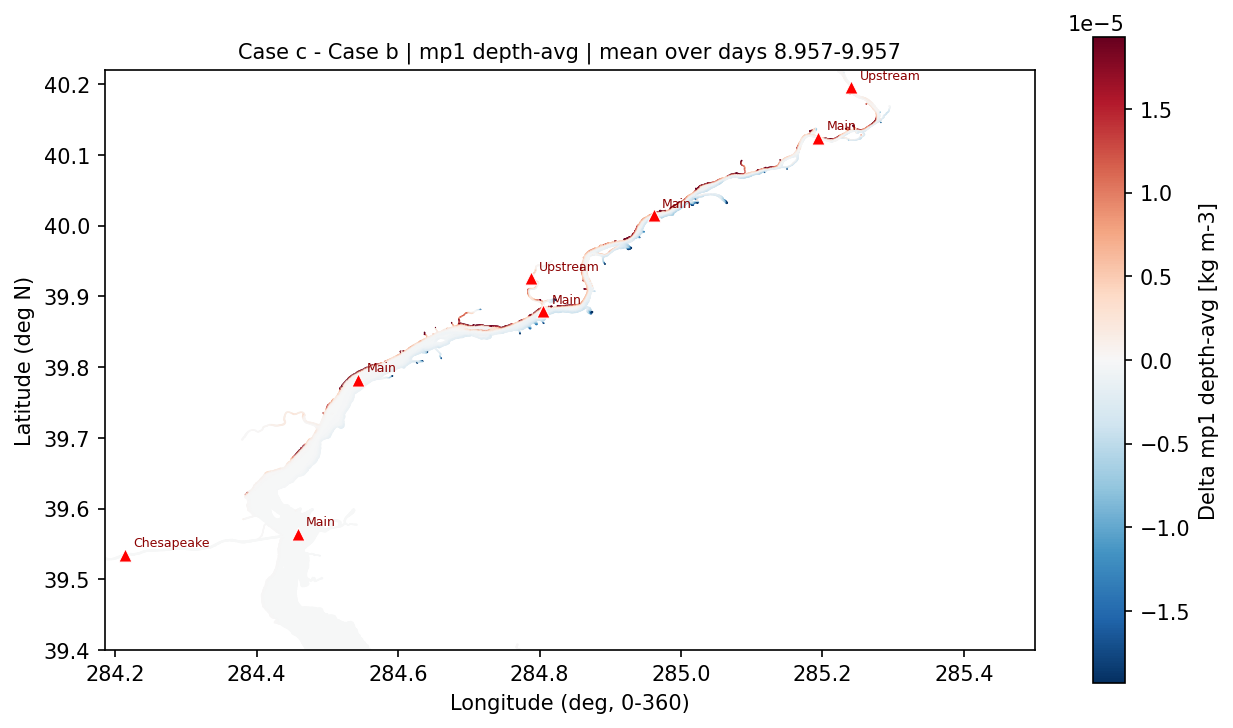
\includegraphics[width=\textwidth]{../FVCOM_MP_test_run/PYTHON/output/spatial_distribution/day10/diff_mp1_davg_casec_minus_caseb.png}
  \caption{Case c $-$ case b}
\end{subfigure}
\caption{Day-mean depth-averaged mp1 difference maps [$\mathrm{kg\,m^{-3}}$],
         final 24~h of the 10-day run.  Diverging colour scale
         (red~=~gain, blue~=~loss).
         \emph{b$-$a}: near-zero everywhere --- cases~a and~b are
         identical (D50~=~0.1~mm, no aggregation).
         \emph{c$-$a} and \emph{c$-$b}: case~c shows elevated
         concentrations near river mouths (stronger local aggregation)
         and reduced concentrations further downstream (faster bed removal).}
\label{fig:diff_mp1}
\end{figure}

% -----------------------------------------------------------------------
\subsection*{R6.\ Station Time Series --- Depth-Averaged mp1}

\begin{figure}[H]
\centering
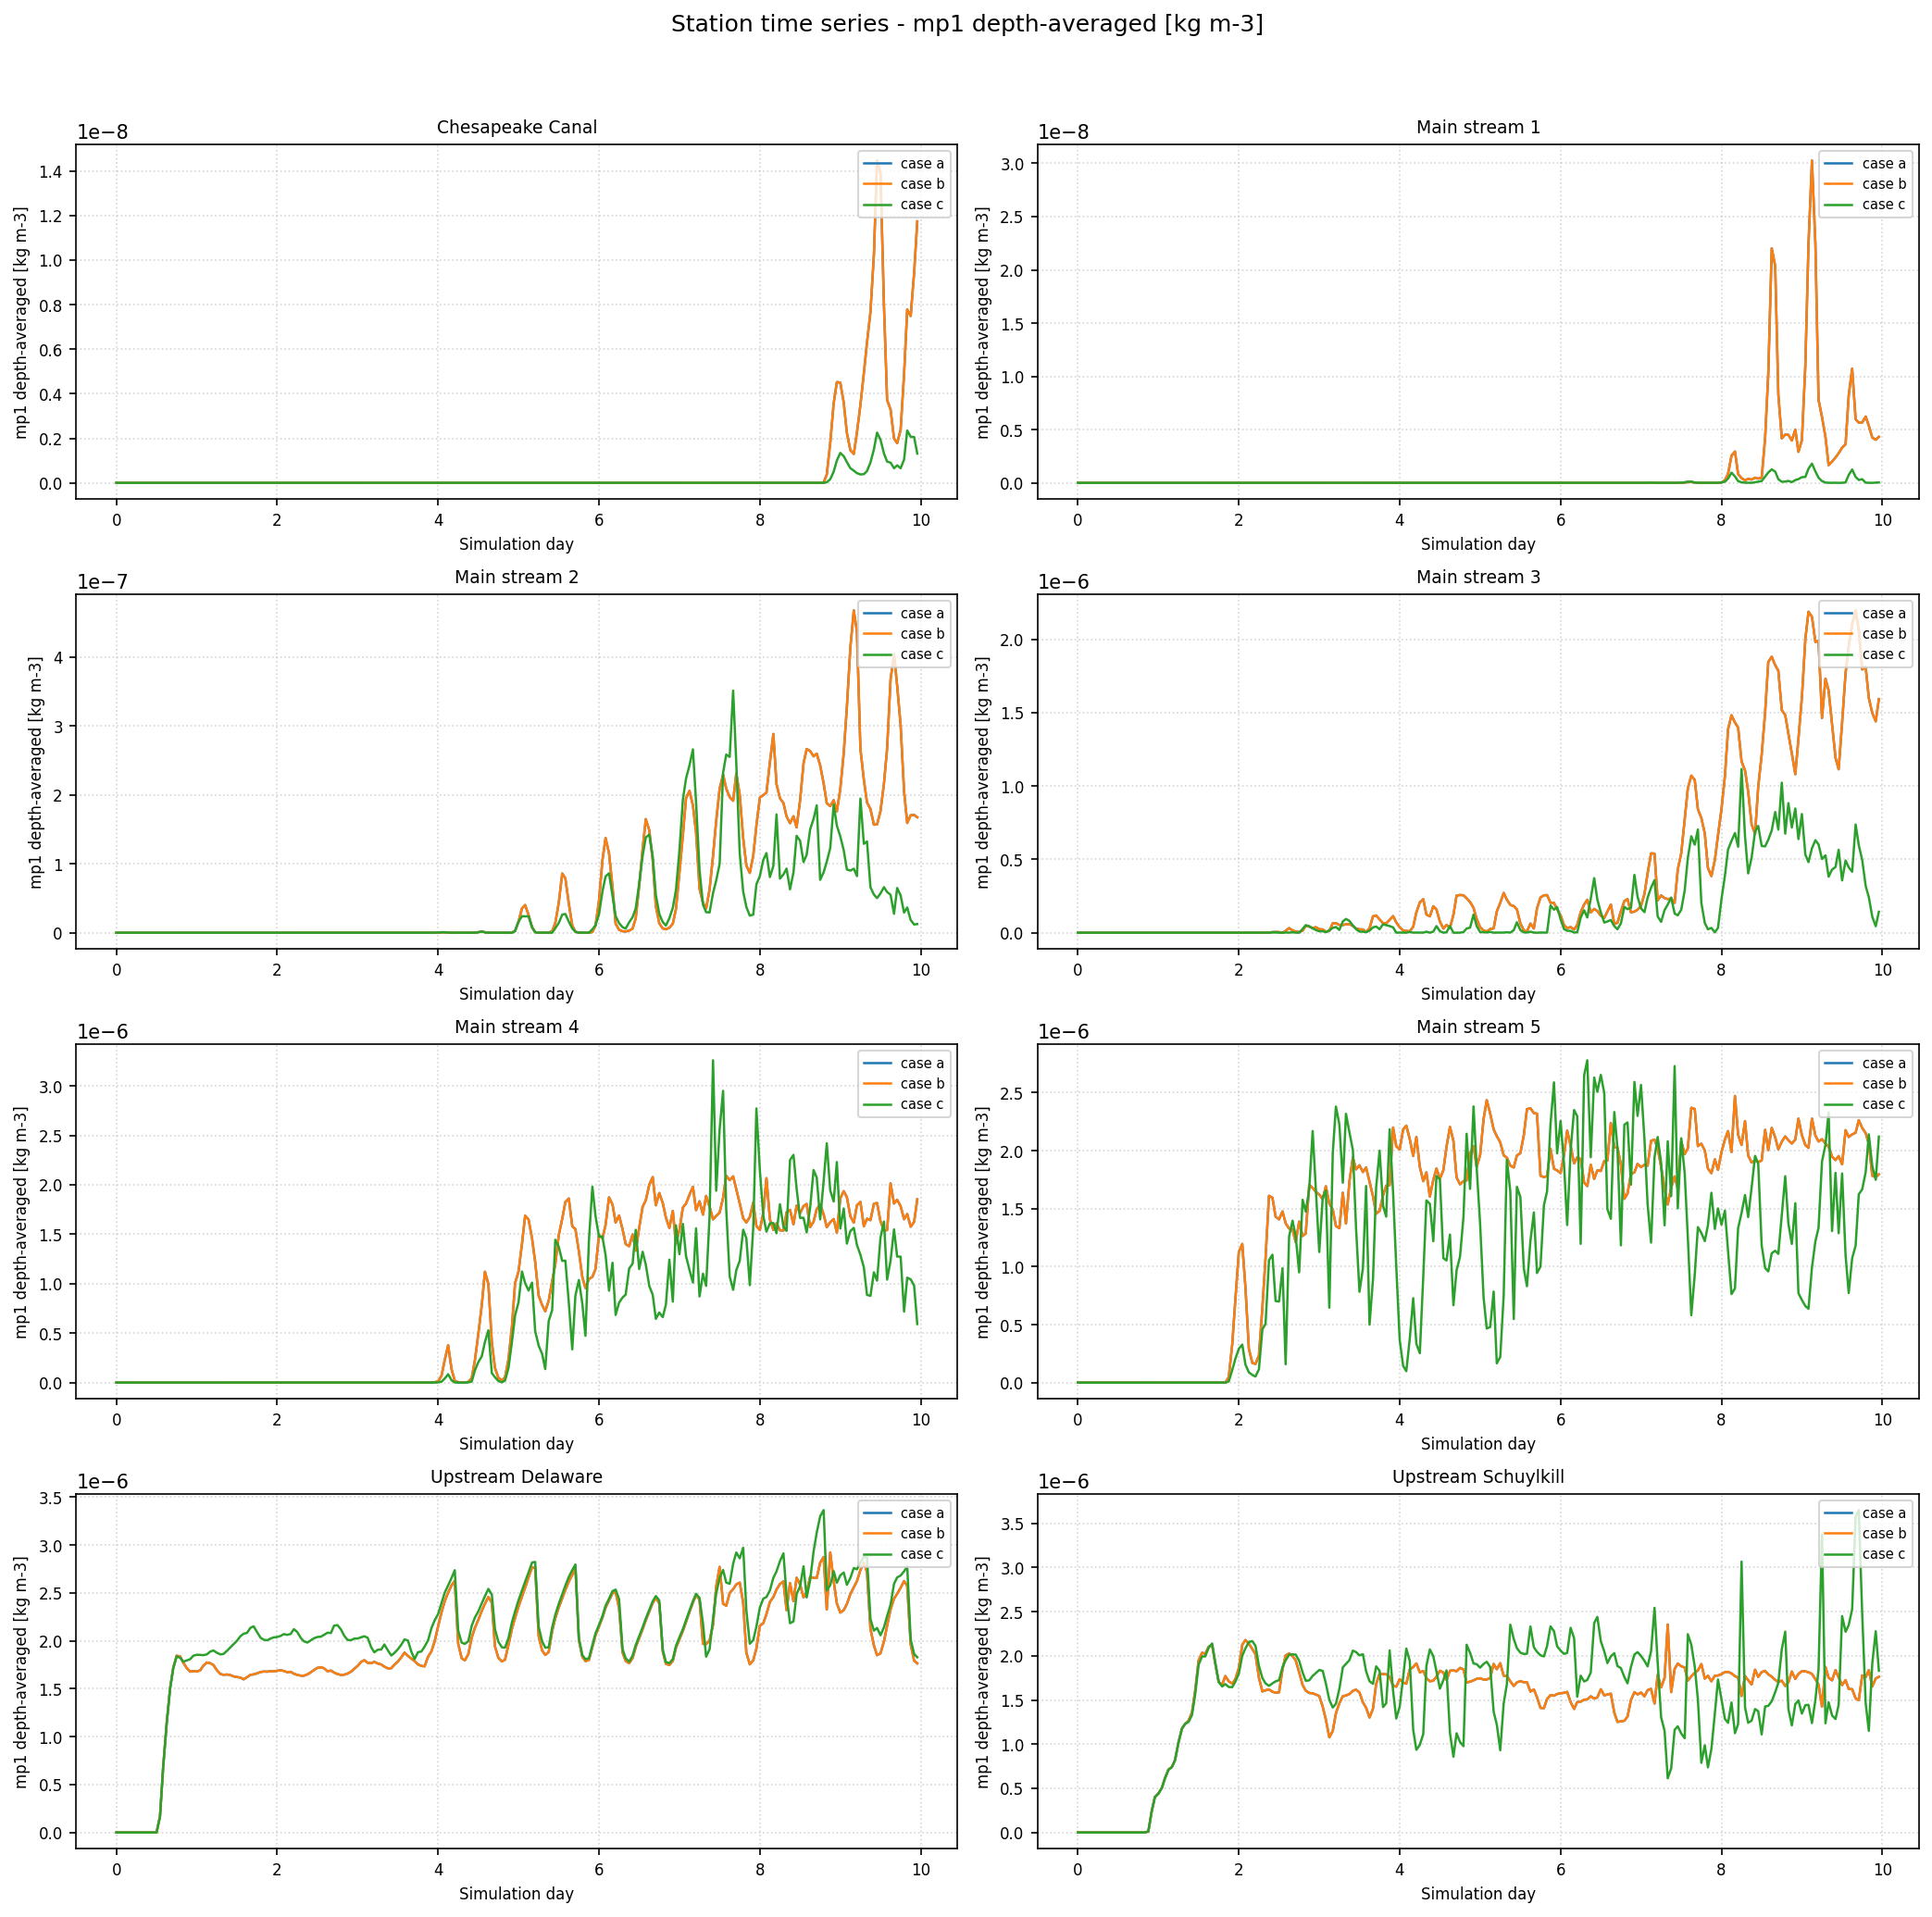
\includegraphics[width=\textwidth]{../FVCOM_MP_test_run/PYTHON/output/spatial_distribution/day10/station_timeseries_mp1_davg.png}
\caption{Depth-averaged mp1 concentration time series at the eight
         monitoring stations over the full 10-day run.
         Blue: case~a (no-floc); orange: case~b (D50~=~0.1~mm);
         green: case~c (D50~=~1.0~mm).
         Cases~a and~b are indistinguishable at all stations.
         Case~c diverges from day~2 onward at the upstream Delaware and
         Schuylkill stations, reflecting the onset of active aggregation
         and bed deposition under the coarser sediment parameterisation.}
\label{fig:station_mp1}
\end{figure}

\section*{Observations}

\begin{enumerate}[(1)]
  \item \textbf{Spatial extent of plastic (all cases).}
        The mp1 plume originates at the river source nodes and disperses
        downstream into the Delaware Bay under tidal forcing.  The plume
        pattern is physically plausible: highest concentrations near the
        Schuylkill confluence and upper Delaware River, decreasing toward
        the bay mouth.
        The pointwise-maximum maps show no isolated hotspot nodes
        disconnected from river sources, confirming the absence of
        localized numerical accumulation.

  \item \textbf{Cases a and b are numerically identical.}
        The b$-$a difference map is uniformly near-zero
        (max $|\Delta|$ $\ll 10^{-5}$~kg\,m$^{-3}$).  With
        D50~=~0.1~mm (fine sediment), the floc kinetic term produces
        no aggregated mass (\texttt{mp1\_agg}~=~0 everywhere in case~b),
        so the \texttt{PLAST\_FLOC=T} path reduces to the same
        behaviour as case~a.

  \item \textbf{Case c shows active aggregation (D50~=~1.0~mm).}
        With coarser sediment, \texttt{mp1\_agg} is non-zero across
        1\,372\,802 node$\times$snapshot combinations
        (peak $1.1\times10^{-3}$~kg\,m$^{-3}$, depth-averaged day-mean).
        The aggregated fraction is spatially co-located with the source
        plume and decays with distance from the river mouths, consistent
        with heteroaggregation driven by local sediment concentration.

  \item \textbf{Bed deposition active only in case c.}
        Cases~a and~b show zero bed mass throughout; case~c accumulates
        bed plastic at 833\,468 nodes (max
        $6.5\times10^{-3}$~kg\,m$^{-2}$), concentrated near the
        upper-bay and tributary junctions where tidal currents slow and
        aggregated particles settle.

  \item \textbf{Elevated water-column peak in case c.}
        The depth-averaged mp1 peak in case~c
        ($3.7\times10^{-3}$~kg\,m$^{-3}$) is $\approx$21$\times$
        higher than in cases~a and~b ($1.7\times10^{-4}$~kg\,m$^{-3}$).
        This reflects the combined effect of slower net settling
        (aggregated particles have altered settling velocity relative to
        free MP) and spatial redistribution by tidal currents before
        deposition.

  \item \textbf{No numerical anomalies detected.}
        No isolated hotspot nodes appear in any pointwise-maximum map.
        The neg-clamp events identified in the checkpoint analysis
        (376 steps, max $1.9\times10^{-4}$~kg/step) produce no
        visible spatial artefacts in the concentration fields.
\end{enumerate}

\section*{Summary and Next Steps}

The spatial distribution analysis confirms that:
\begin{itemize}
  \item The mp1 plume is physically plausible and free of numerical
        accumulation artefacts in all three cases.
  \item Cases~a and~b are numerically identical under the current
        parameterisation (\texttt{SOURCE\_AG\_RATE}~=~0, D50~=~0.1~mm);
        no aggregation or bed deposition occurs.
  \item The corrected case~c (D50~=~1.0~mm) demonstrates the full
        floc-interaction pathway: active aggregation
        (\texttt{mp1\_agg} $> 0$ domain-wide), bed deposition at
        $\sim$56\% of nodes, and a 21$\times$ higher peak water-column
        concentration relative to cases~a and~b.
  \item Fix~B\texttt{+} (Memo~04) maintains mass conservation with
        active kinetics; the split-consistency error
        $|\texttt{mp1\_agg}+\texttt{mp1\_dis}-\texttt{mp1}|$ remains
        at machine precision ($< 3\times10^{-7}$~kg domain-wide).
\end{itemize}

Potential next steps:
\begin{itemize}
  \item Extended 30-day runs (confirmed to be mass-conservative per Memo~04)
        to verify longer-term spatial spreading and floc-component evolution.
  \item Open-boundary hypothesis testing: instrument OBC fluxes at the
        southern bay mouth to quantify tidal export of plastic.
  \item Fix~D: multi-species flux limiting when \texttt{SOURCE\_AG\_RATE} $> 0$
        causes \texttt{conc\_a} $> 0$, which is excluded from the current
        10-day tests but required for full-physics runs.
\end{itemize}

\end{document}
